\begin{figure}[hb]
    \centering
    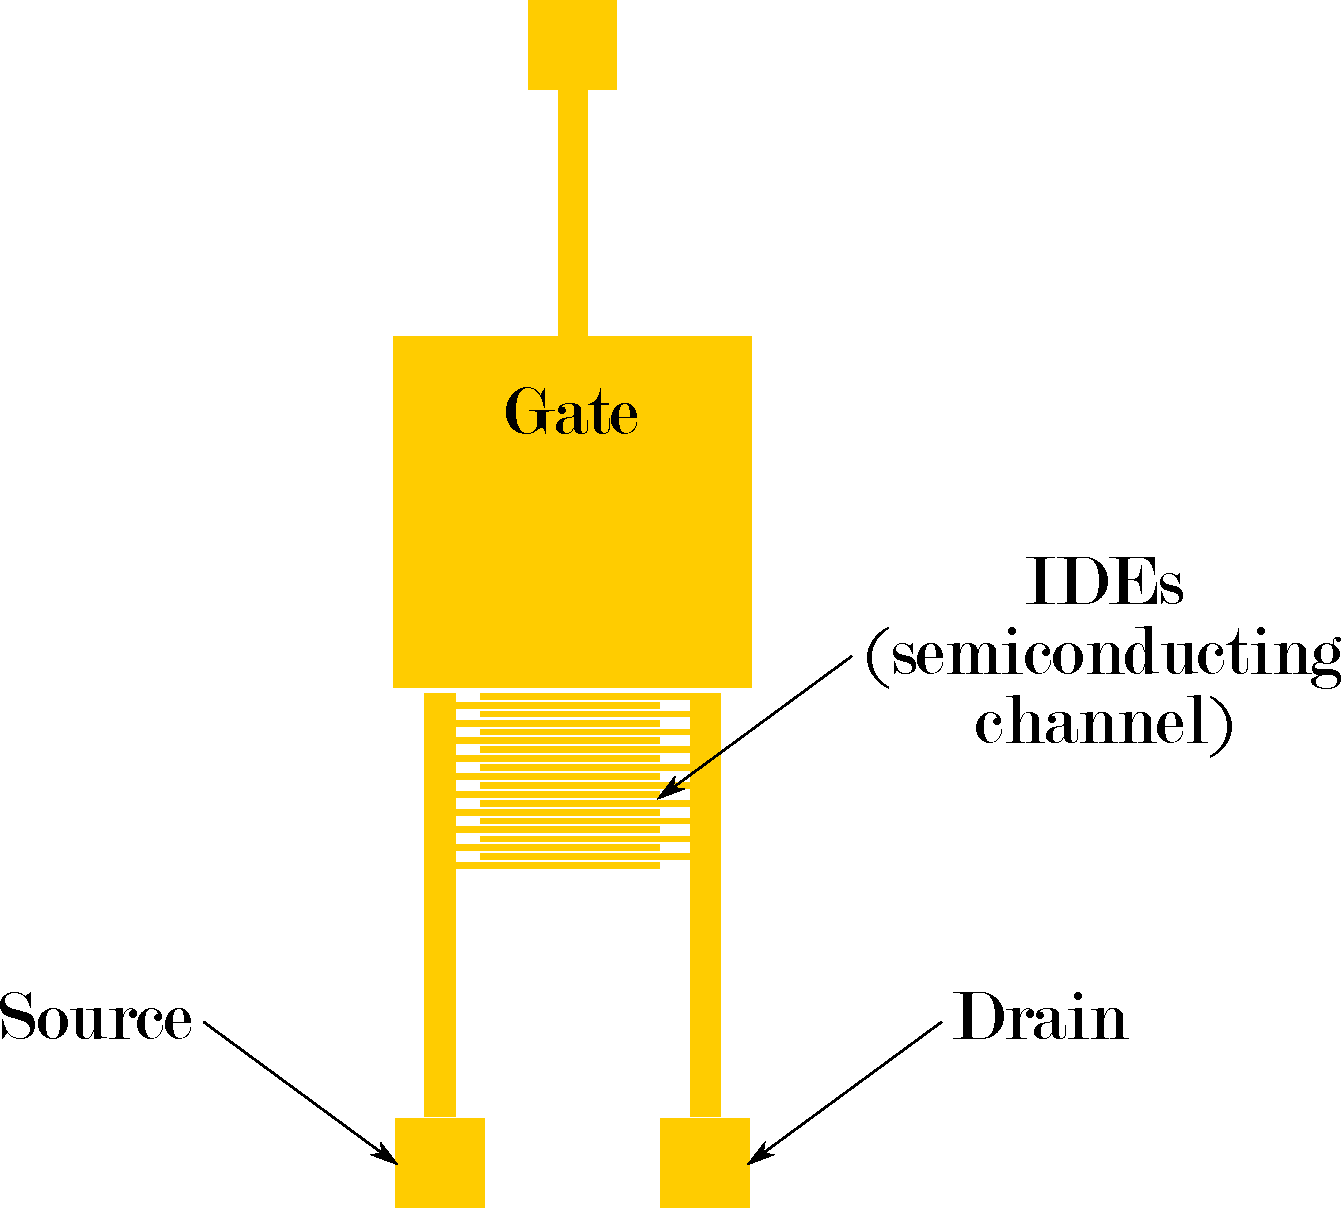
\includegraphics[width = 0.3\textwidth]{figures/chapter3/sdEGFET/sdEGFET_scheme.pdf}
    \caption{Illustration of an EG-FET with a reduced distance between the gate and the channel. The other dimensions of the device remained unchanged: the gate is \SI{5.7}{\mm} $\times$ \SI{5.7}{\mm} big, the channel length is \SI{50}{\um}, the arm height is \SI{100}{\um}, the arm length is \SI{3}{\mm}. The only parameter changed is the distance between the gate and the channel, which is reduced to \SI{100}{\um}.}
\end{figure}

After testing a known structure, an attempt was made to change the geometry to test its impact on stability and to try to develop faster stabilizing and more stable devices. In this case, the channel of the standard EG-FET was repositioned closer to the gate, reducing the distance from \SI{1.5}{\mm} to \SI{100}{\um}, resulting in what is herein referred to as the \vv{small distance} EG-FET, or sdEG-FET. The hypothesis behind this change is that reducing the channel-gate distance could allow the gate to have greater control over the channel, potentially leading to faster stabilization compared to the standard geometry tested in Section \ref{sec:big_channel}. This section aims to evaluate the validity of this hypothesis by analyzing the transfer curves, normalized current, and other relevant parameters collected for the standard device, with and without the membrane.

\begin{figure}
    \centering
    \subfloat[Transfer characteristics]{
        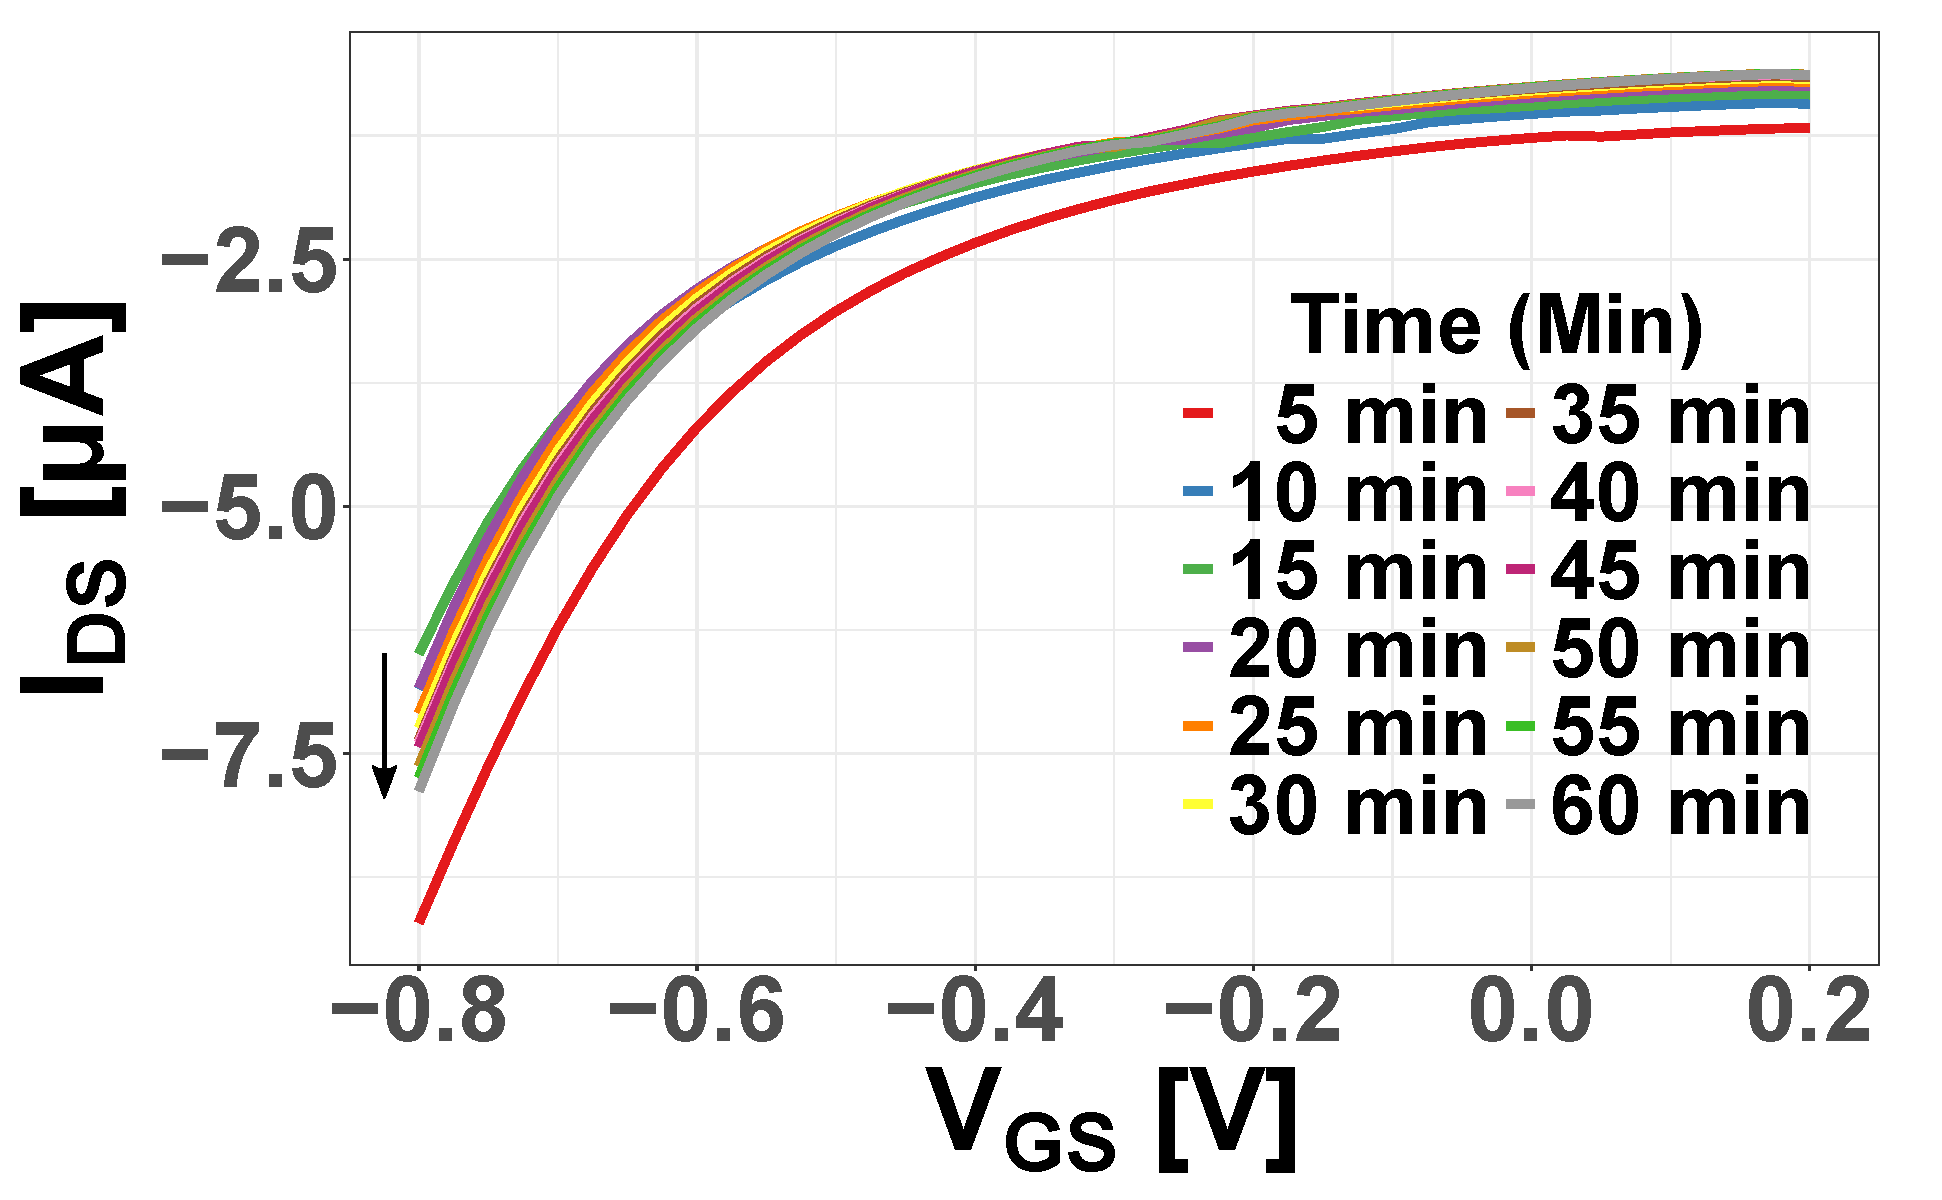
\includegraphics[width=0.45\textwidth]{figures/chapter3/sdEGFET/sdTransfer.pdf}
        \label{fig:sdTransfer}
    }
    \hfill
    \subfloat[Normalized current]{
        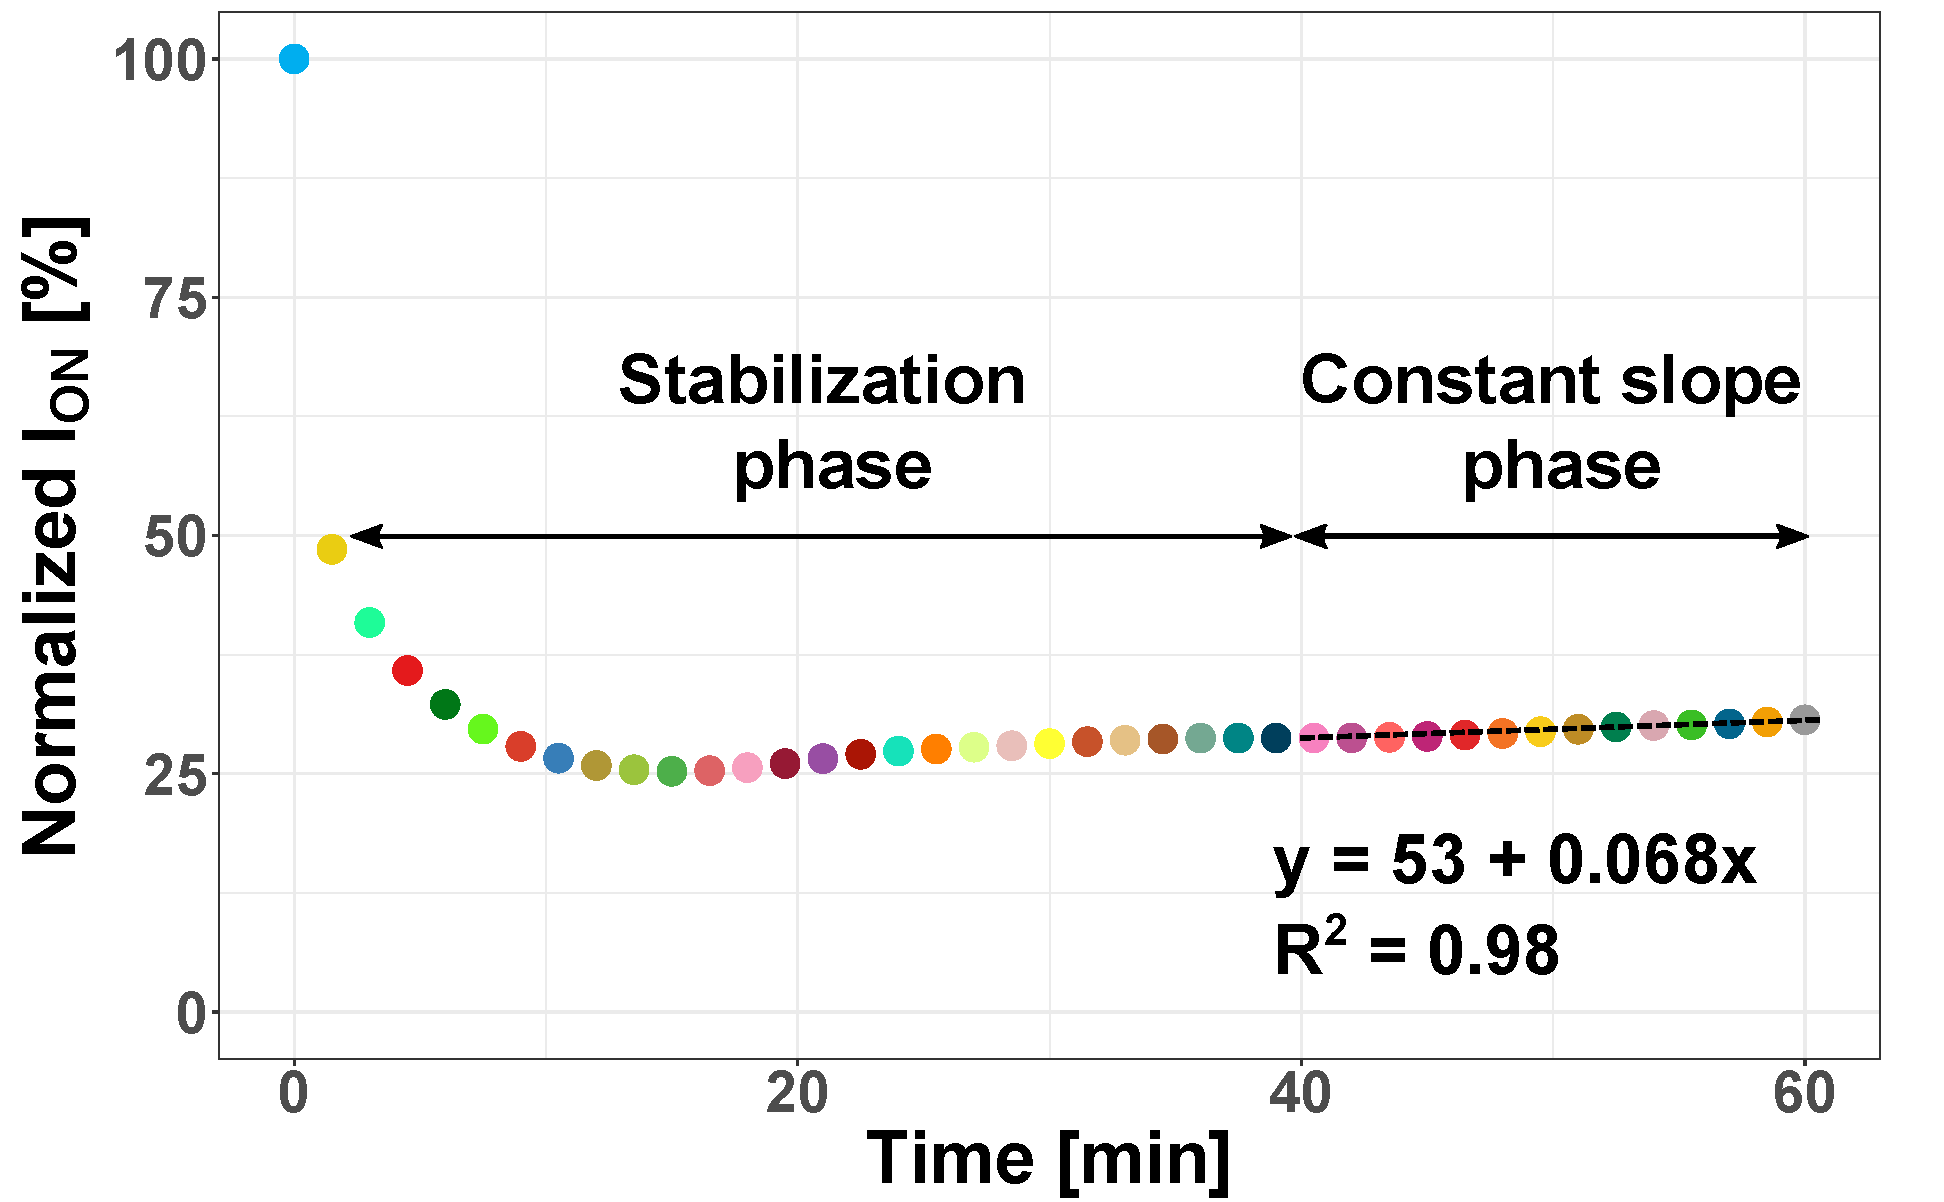
\includegraphics[width=0.45\textwidth]{figures/chapter3/sdEGFET/sdNormalized.pdf}
        \label{fig:sdNormalized}
    }
    \caption{The figure displays
    (a) the transfer characteristics and 
    (b) the normalized current extracted from the transfer characteristics for a sdEG-FET. When compared to the results previously obtained, the behavior is very similar: initially, there is a \emph{stabilization phase}, during which the current is highly variable and no clear trend is visible. However, after this phase, the system finds an equilibrium, entering the \emph{constant slope phase} where the current is linear with respect to time.}
    \label{fig:sdData}
\end{figure}

The transfer characteristics collected for the encapsulated sdEG-FET (Figure \ref{fig:sdTransfer}) show a trend similar to that of the standard EG-FET. Specifically, the first transfer curve is the one at the highest current, the following ones are much lower, but then begin to increase again over time, as it was observed for the standard device. This is confirmed by observing the normalized current (Figure \ref{fig:sdNormalized}), which follows a similar pattern. The first half of the measurement is characterized by a \emph{stabilization phase}, where the current fluctuates, indicating that the system is undergoing changes that should lead toward an equilibrium. After this, the \emph{constant slope phase} is visible, where the current follows a linear trend and the system stabilizes. 

Data analysis was conducted as before, thus evaluating the point in time when the current trend becomes linear with respect to time with $R^2>0.98$.
From this, it was concluded that the sdEG-FET reaches equilibrium on average after \SI{41}{}$\pm$\SI{3}{\min} ($N = 5$). This result proved that the initial hypothesis was incorrect: reducing the channel-to-gate distance does not accelerate the stabilization process.

\begin{figure}
    \centering
    \subfloat[\igs{} and \ids{} of an sdEG-FET]{
        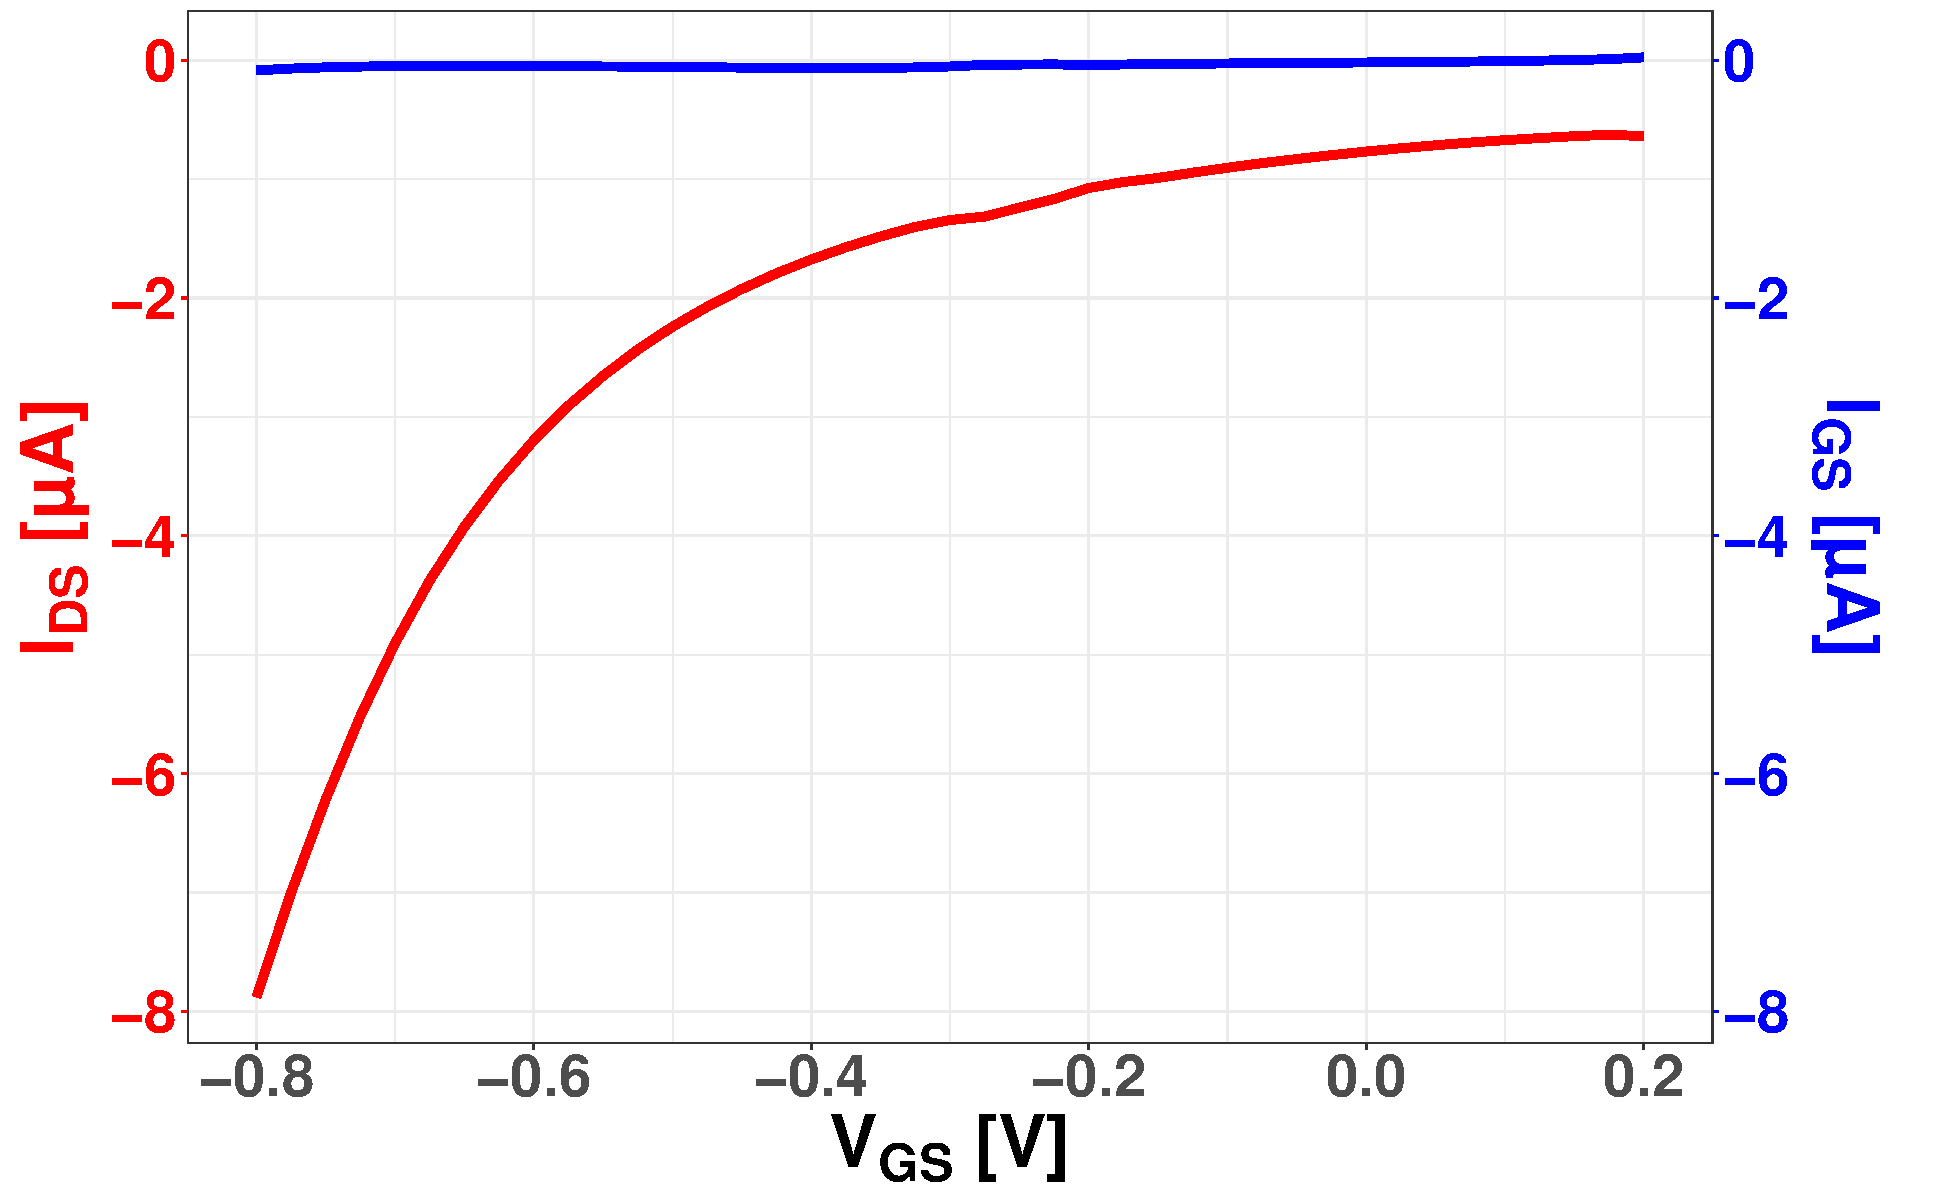
\includegraphics[width = 0.45\textwidth]{figures/chapter3/sdEGFET/sdIdIgCurves.pdf}
        \label{fig:sdIdIgCurves}
    }
    \hfill
    \subfloat[Hysteresis of an sdEG-FET]{
        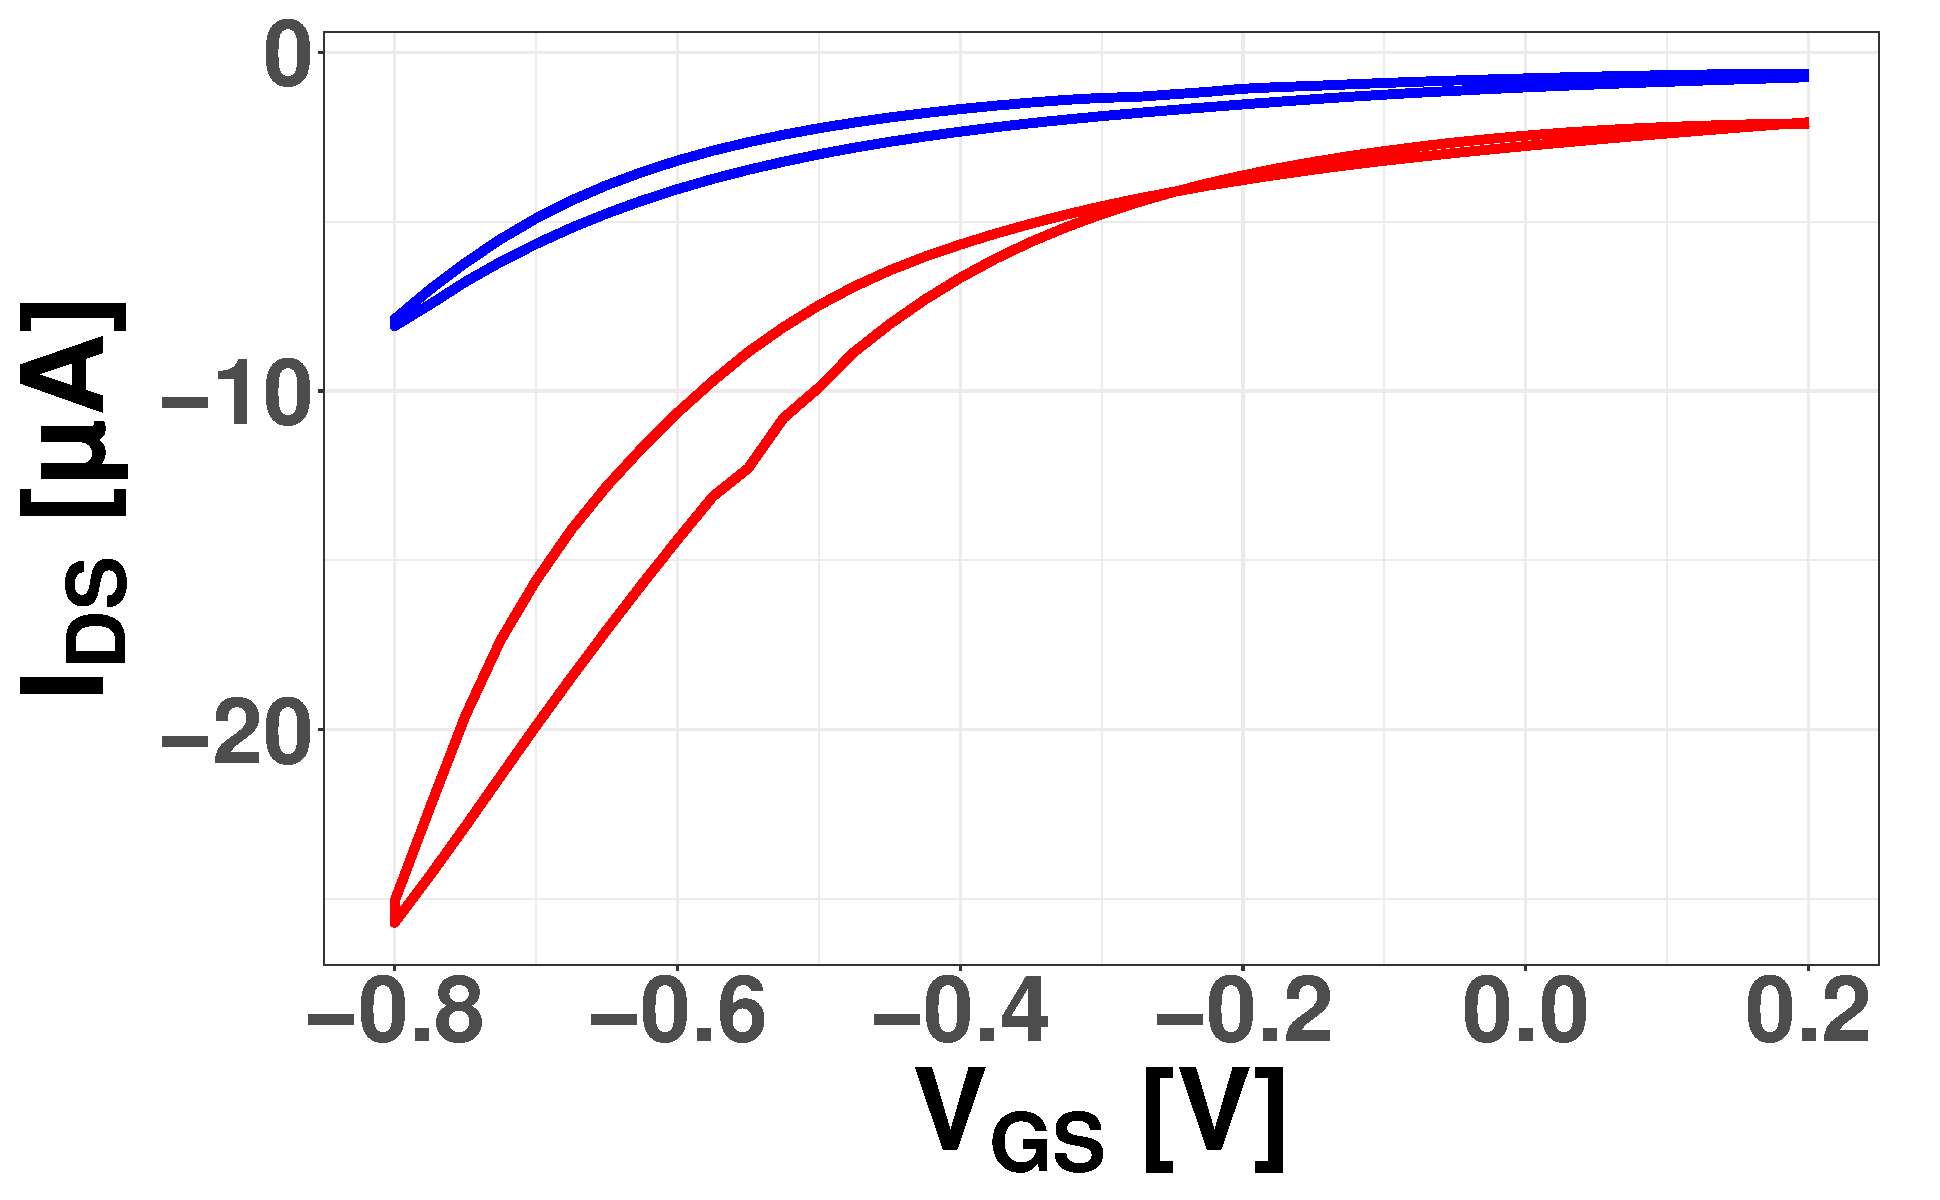
\includegraphics[width = 0.45\textwidth]{figures/chapter3/sdEGFET/sdHysteresis.pdf}
        \label{fig:sdHysteresis}
    }
    \caption{\note{Further electrical characterization of an sdEG-FET.
    (a) \igs{} and \ids{}: the \igs{} is orders of magnitude lower than the \ids{}, similar to the behavior of standard EG-FETs with membrane encapsulation. This indicates that there is still minimal leakage current, even though gate and channel are much closer to each other. 
    (b) Hysteresis decreases from \SI{0.075}{\V} at \SI{0}{\min} to \SI{-0.05}{\V} at \SI{60}{\min}, showing a worse performance compared to the standard EG-FET, both with and without the membrane.}}
    \label{fig:sdParameters}
\end{figure}

Following this preliminary characterization, additional analyses were conducted. In particular, the \ids{} and \igs{} of the sdEG-FET are displayed in Figure \ref{fig:sdIdIgCurves}: the trend is similar to that of the standard EG-FET, with the curves displaying the typical behavior, \ie{} the \igs{} is orders of magnitude lower than the \ids{}. On the other hand, a difference can be observed in the hysteresis plot (Figure \ref{fig:sdHysteresis}): Unlike the standard EG-FET, where the hysteresis approaches \SI{0}{\V} after \SI{60}{\min} of measurements, the sdEG-FET has a residual hysteresis of \SI{-0.05}{\V}.  This could be attributed to the reduced channel-to-gate distance: the supposed increased gate control over the channel might introduce additional issues, such as an altered electrostatic environment that could prevent the voltage from going to zero. Indeed, when the gate is closer to the channel the charge trapping could have a bigger impact, leading to a higher hysteresis.

\begin{figure}
    \centering
    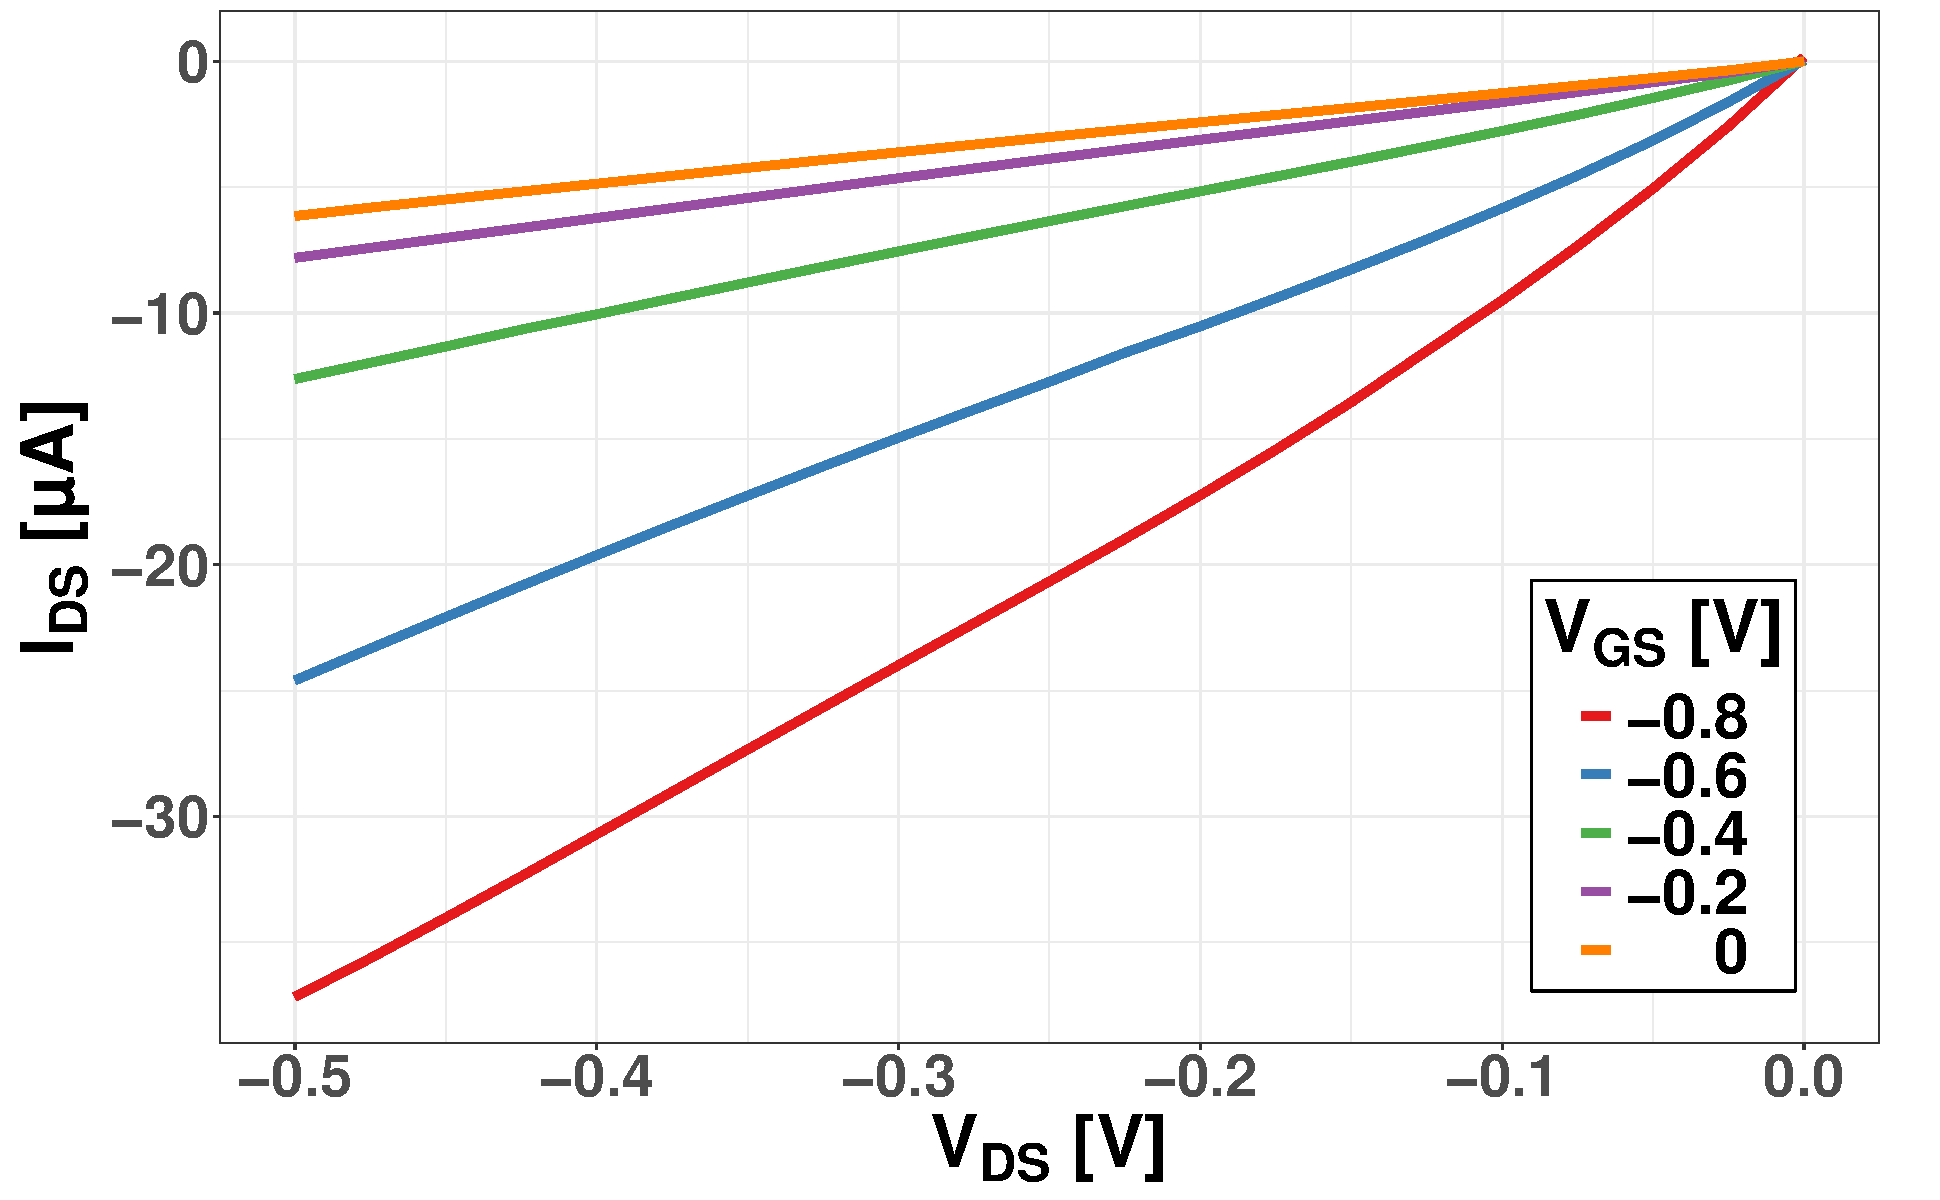
\includegraphics[width = 0.45\textwidth]{figures/chapter3/sdEGFET/sdOutput.pdf}
    \caption{Electrical characterization of an sdEG-FET.
        Output characteristics: these curves show the behavior of a device that operates in linear regime, similarly to the encapsulated EG-CNTFET. Indeed, the device does not approach saturation.}
    \label{fig:sdOutput}
\end{figure}

As it was done before, the output characteristics were collected and analyzed. The output characteristics of the sdEG-FET are similar to those of the standard EG-FET with the protective membrane on the channel. Indeed, it is observed that sdEG-FET does not reach saturation and instead operates in the linear mode.
This implies that the device is not achieving its theoretical maximum output current, which typically occurs in the saturation region. In this region, the \ids{} is proportional to both \vgs{} and \vds{}, making it suitable for analog and low-power operations. This proportionality allows to control the current flow, being beneficial for those applications that require continuous modulation of the output signal. Moreover, working in this regime allows small variations of \vgs{} to effectively modulate the \ids{}, thus reducing energy consumption. This can be advantageous in the context of sensors, where operating in the linear regime ensures a predictable relationship between the \vgs{} and the \ids{}, facilitating signal processing. However, this also means that the device is not achieving its theoretical maximum output current, which typically occurs in the saturation region. Furthermore, this regime is more affected by contact resistance, which can influence device performance and limit current drive capabilities, potentially impacting the sensitivity and reliability of sensor measurements.

\begin{figure}
    \centering
    \subfloat[ON/OFF ratio for the three devices]{
        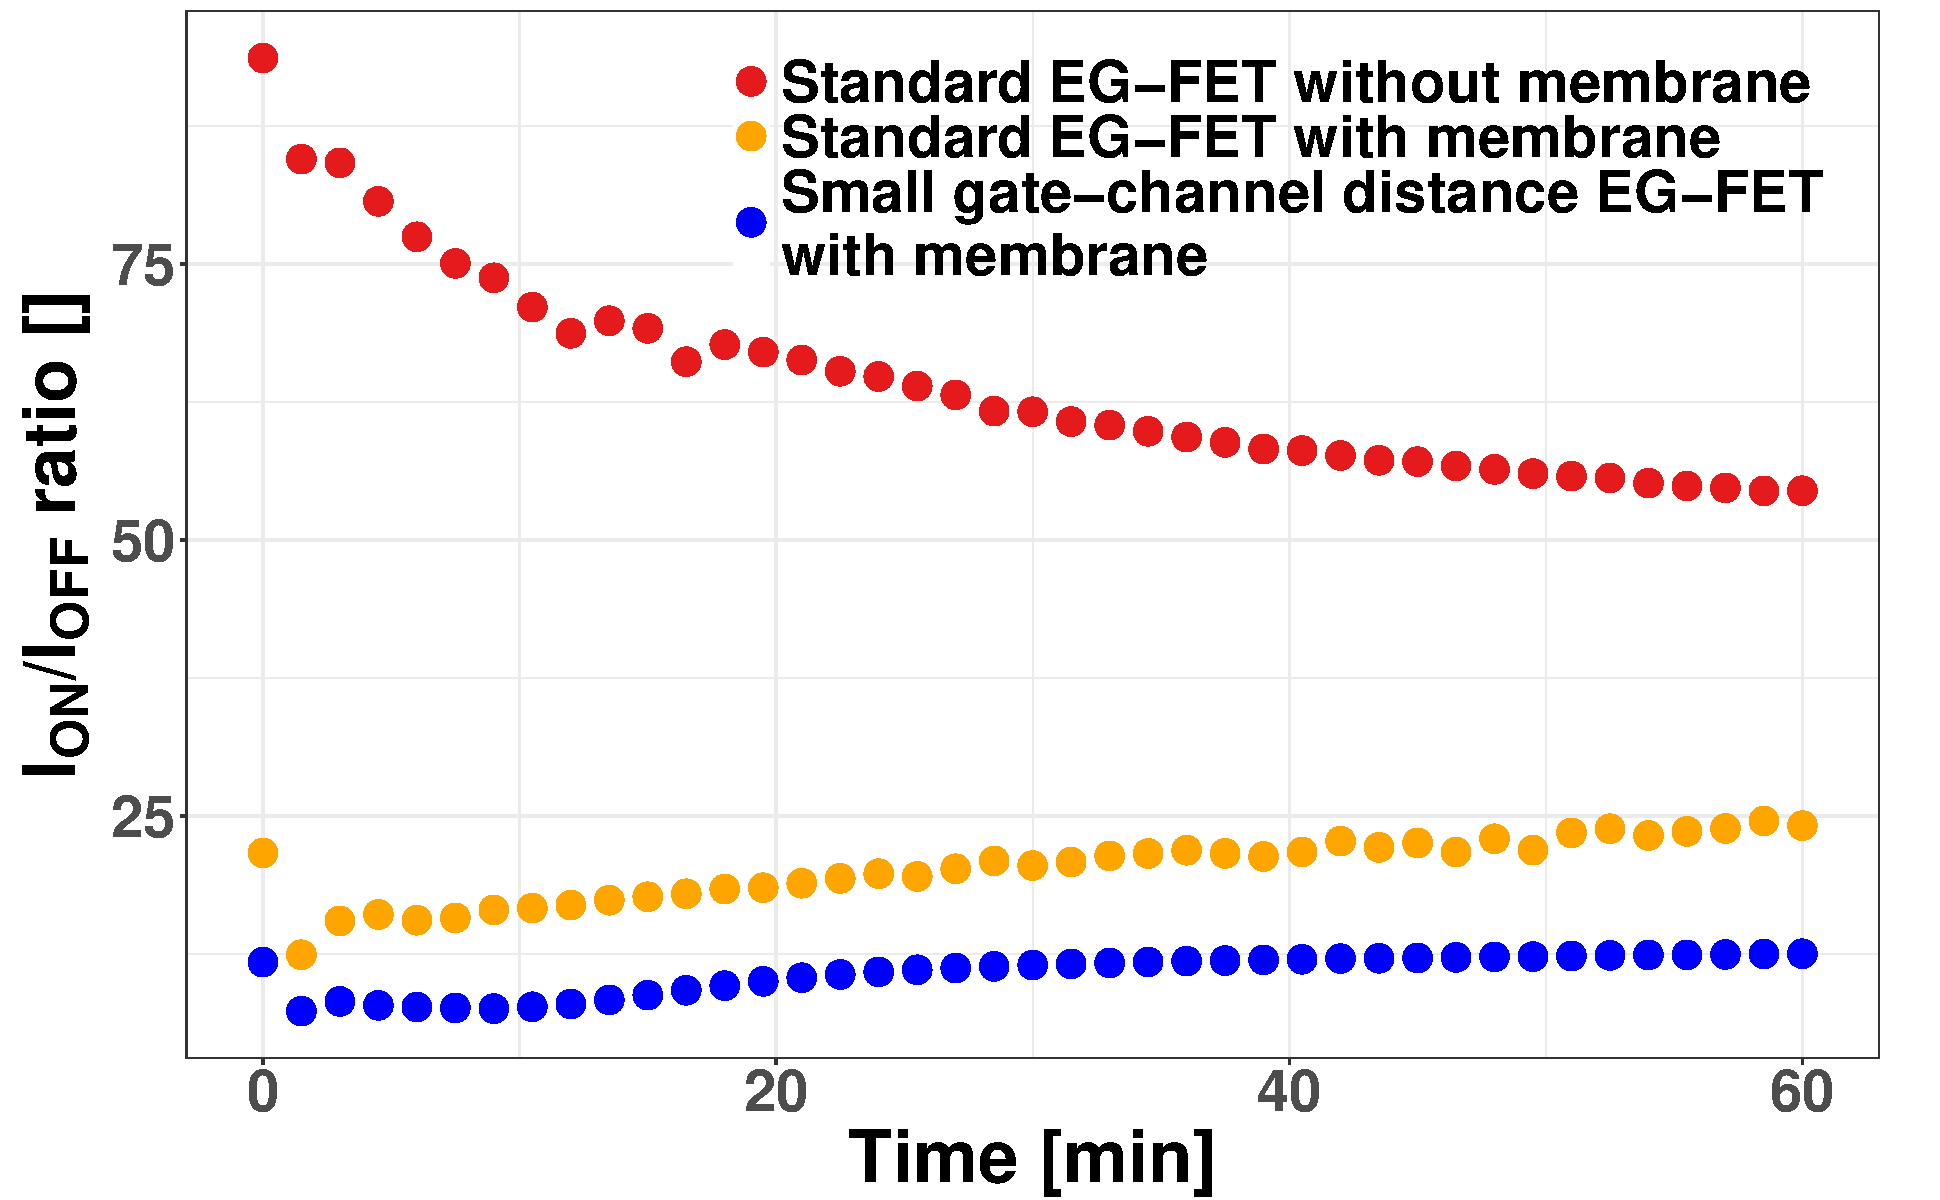
\includegraphics[width = 0.45\textwidth]{figures/chapter3/sdEGFET/sdOnOffRatio.pdf}
        \label{fig:sdOnOffRatio}
    }
    \hfill
    \subfloat[\vth{} for the three devices]{
        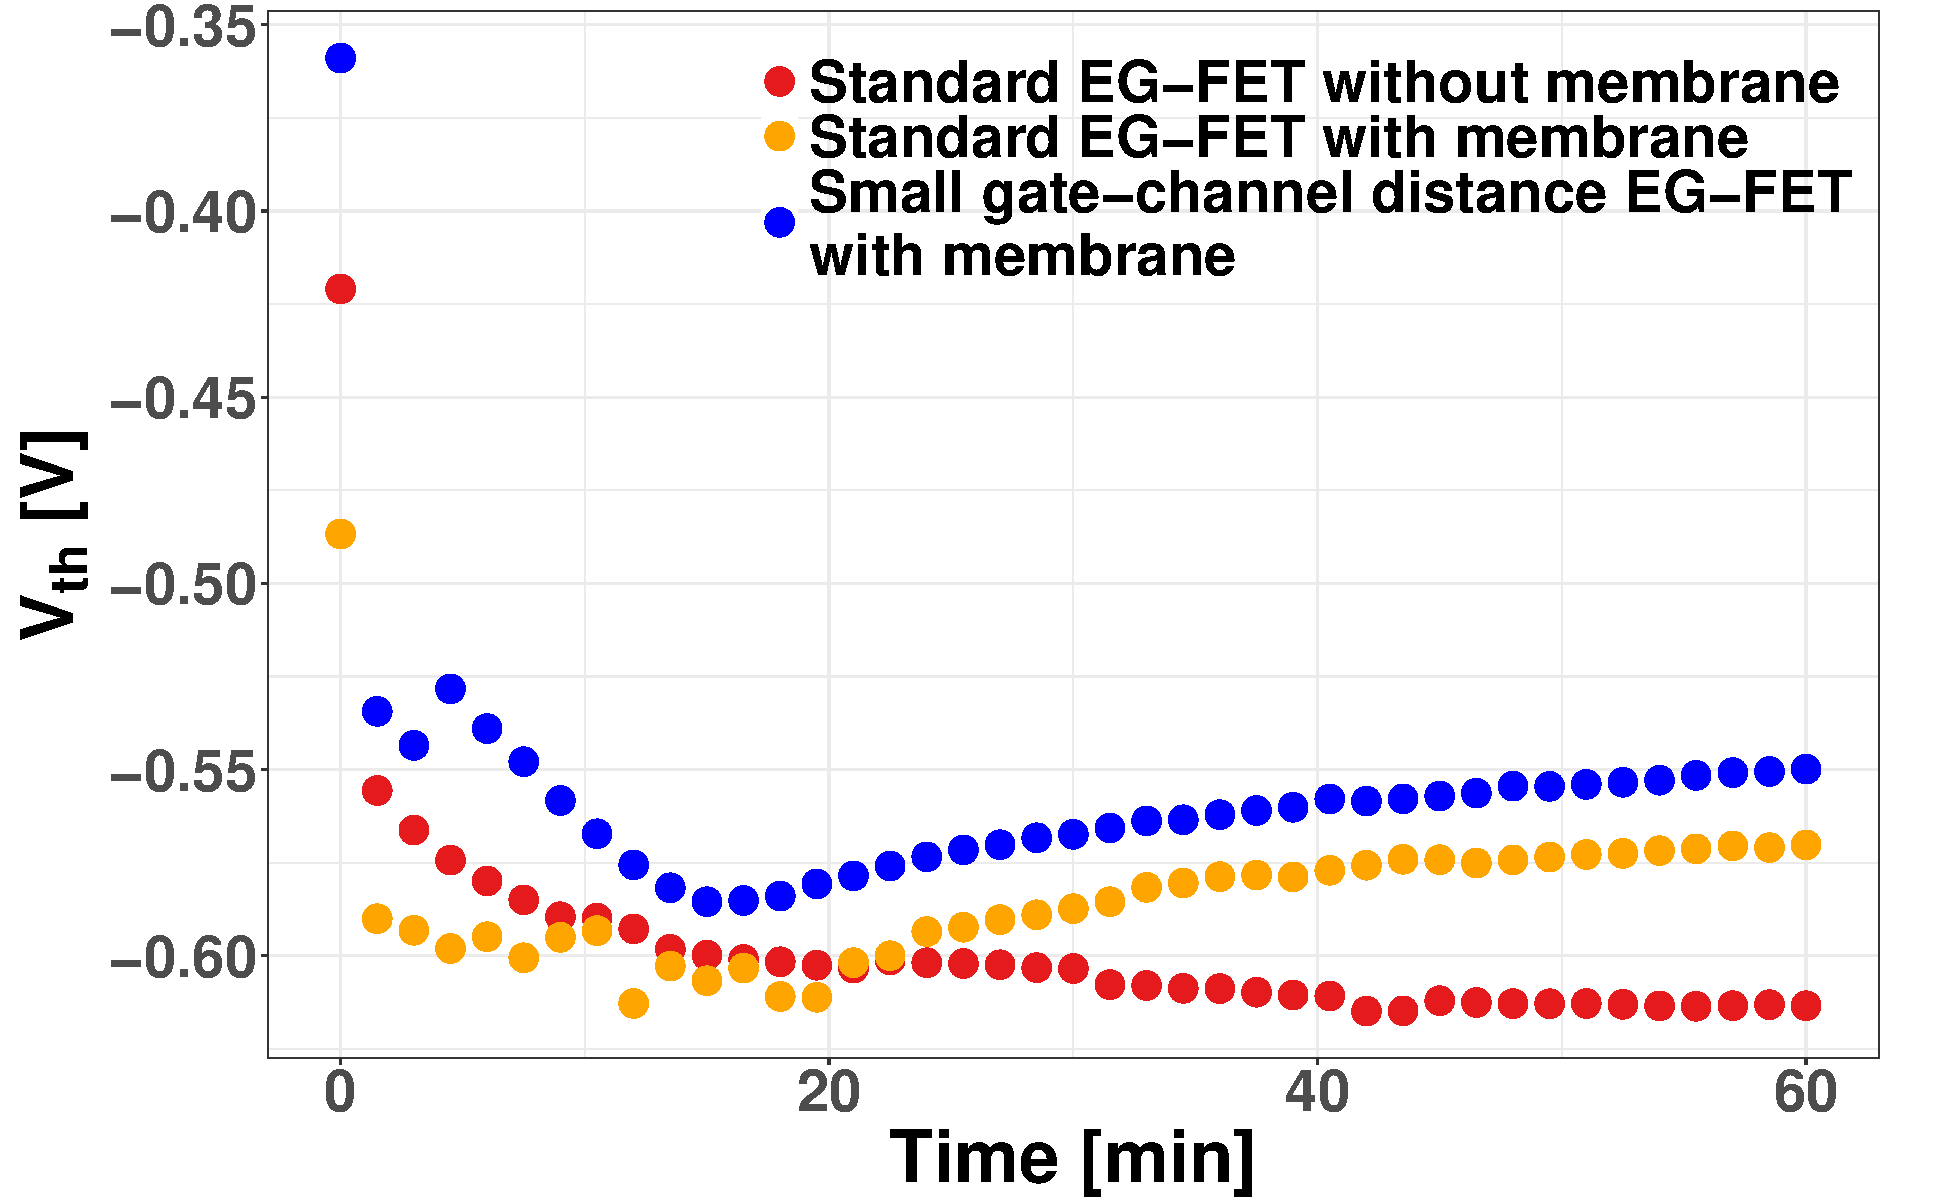
\includegraphics[width = 0.45\textwidth]{figures/chapter3/sdEGFET/sdVth.pdf}
        \label{fig:sdVth}
    }
    \caption{Comparison of the average of electrical parameters.
        (a) ON/OFF ratio trends for the three devices described so far, \ie{} the standard bare EG-CNTFET in red, the standard EG-CNTFET with the encapsulated channel in yellow and the sdEG-FET in blue. This image shows that the sdEG-FET has the lowest ratio among the devices, indicating the worst performance. 
        (b) \vth{} exhibits the lowest values throughout the measurements for the sdEG-FET, suggesting a more efficient device with lower power consumption.}
    \label{fig:avgSdParams}
\end{figure}

Further characterization of the behaviour of sdEG-FETs required calculating additional parameters. In particular, the ON/OFF ratio and the \vth{} were calculated and a comparison was made with the same parameters of the standard EG-FET, both with and without the lipophilic membrane.

Figure \ref{fig:sdOnOffRatio} shows that the ON/OFF ratio of the sdEG-FET follows the same trend as the EG-FET with the membrane, continually increasing over time, thus indicating an improvement in performance. However, the value is slightly lower for the sdEG-FET compared to the standard EG-FET, suggesting that it is slightly less performing.

On the other hand, the threshold voltage (\vth{}) of the sdEG-FET is lower compared to the EG-FET with the membrane, yet still following the same decreasing trend over time. This is a indication of a slightly bettere performance, as a lower \vth{} leads to reduced power consumption, which could help develop energy-efficient devices. Additionally, a lower \vth{} indicates an enhanced device switching speed and a lower voltage required to turn the device on; this characteristic is beneficial when the final goal for the device is the development of a sensor, indeed a higher switching speed would improve the responsiveness of the platform.

Considering all the factors discussed above, the conclusion is that while the performance of the sdEG-FET is not necessarily poor, the standard EG-CNTFET with the membrane is better. Indeed, the standard EG-CNTFET is faster in reaching equilibrium and is easier to work with. The smaller channel-to-gate distance in the sdEG-FET makes it challenging to dropcast the membrane without compromising the gate. If the gate is partially covered, the charge accumulation is altered, leading to reduced control over the channel and a subsequent decrease in the output current. Therefore the sdEG-FET does not present an ideal solution for our sensing applications.
